% !TEX root = ../../main.tex
\chapter{Metodologi Penelitian}

Bab ini menjelaskan tahapan penelitian yang digunakan untuk mengevaluasi karakteristik operasi relay 21 dan relay 87L pada sistem transmisi dengan integrasi \textit{inverter-based resources} (IBR). Penelitian dilakukan melalui simulasi pada DIgSILENT PowerFactory. Variabel utama yang dibandingkan adalah jenis IBR, yaitu \textit{wind turbine type 3}, \textit{wind turbine type 4}, dan \textit{photovoltaic}, sedangkan setting proteksi dipertahankan berdasarkan kondisi sistem konvensional.

\section{Diagram Alir Penelitian}

Alur penelitian ditunjukkan pada Gambar \ref{fig:flowchart_tahapan_penelitian}. Tahapan penelitian diawali dengan studi literatur mengenai karakteristik IBR, prinsip kerja relay 21, prinsip kerja relay 87L, serta pengaruh IBR terhadap proteksi saluran transmisi. Hasil studi literatur digunakan sebagai dasar untuk menentukan ruang lingkup simulasi, parameter yang diamati, dan cara membaca respons relay.

\usetikzlibrary{shapes.geometric, arrows.meta, positioning}

\begin{figure}[H]
    \centering
    \resizebox{0.25\textwidth}{!}{%
        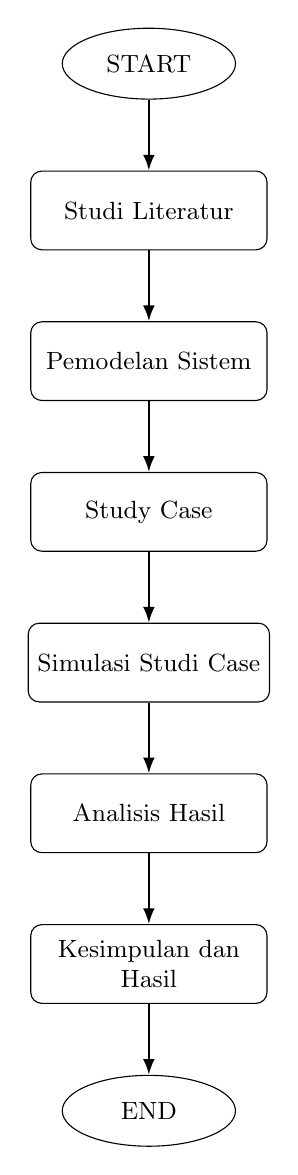
\begin{tikzpicture}[
            node distance=0.9cm,
            every node/.style={font=\small},
            startstop/.style={
                    ellipse,
                    draw,
                    minimum width=2.2cm,
                    minimum height=0.9cm,
                    align=center
                },
            process/.style={
                    rectangle,
                    rounded corners,
                    draw,
                    minimum width=3.0cm,
                    minimum height=1.0cm,
                    align=center
                },
            arrow/.style={
            -{Latex[length=2mm]},
            thick
            }
            ]

            % Node flowchart
            \node (start) [startstop] {START};

            \node (literatur) [process, below=of start] {Studi Literatur};

            \node (model) [process, below=of literatur] {Pemodelan Sistem};

            \node (studycase) [process, below=of model] {Study Case};

            \node (simulasi) [process, below=of studycase] {Simulasi Studi Case};

            \node (analisis) [process, below=of simulasi] {Analisis Hasil};

            \node (kesimpulan) [process, below=of analisis] {Kesimpulan dan\\Hasil};

            \node (end) [startstop, below=of kesimpulan] {END};

            % Garis panah
            \draw [arrow] (start) -- (literatur);
            \draw [arrow] (literatur) -- (model);
            \draw [arrow] (model) -- (studycase);
            \draw [arrow] (studycase) -- (simulasi);
            \draw [arrow] (simulasi) -- (analisis);
            \draw [arrow] (analisis) -- (kesimpulan);
            \draw [arrow] (kesimpulan) -- (end);

        \end{tikzpicture}%
    }
    \caption{Diagram Alir Penelitian}
    \label{fig:flowchart_tahapan_penelitian}
\end{figure}

Setelah studi literatur, penelitian dilanjutkan dengan pemodelan sistem pada DIgSILENT PowerFactory. Model sistem digunakan untuk membentuk kondisi acuan tanpa IBR dan kondisi dengan integrasi IBR. Diagram alir menunjukkan bahwa terdapat kondisi tanpa IBR dan beberapa skenario IBR yang kemudian disimulasikan. Setiap skenario dijalankan untuk memperoleh data respons relay, kemudian hasilnya dianalisis untuk menyusun kesimpulan dan rekomendasi teknis.

\section{Model Sistem dan Asumsi Studi}

Model sistem yang digunakan dalam penelitian ini merupakan model sistem \textit{modified two-area kundur system} pada DIgSILENT PowerFactory sebagaimana ditunjukkan pada Gambar \ref{fig:sld_pf}. Model tersebut memuat beberapa bus, saluran transmisi, sumber konvensional, beban, shunt atau filter, serta unit IBR yang terhubung ke jaringan melalui transformator.

\begin{figure}[H]
    \centering
    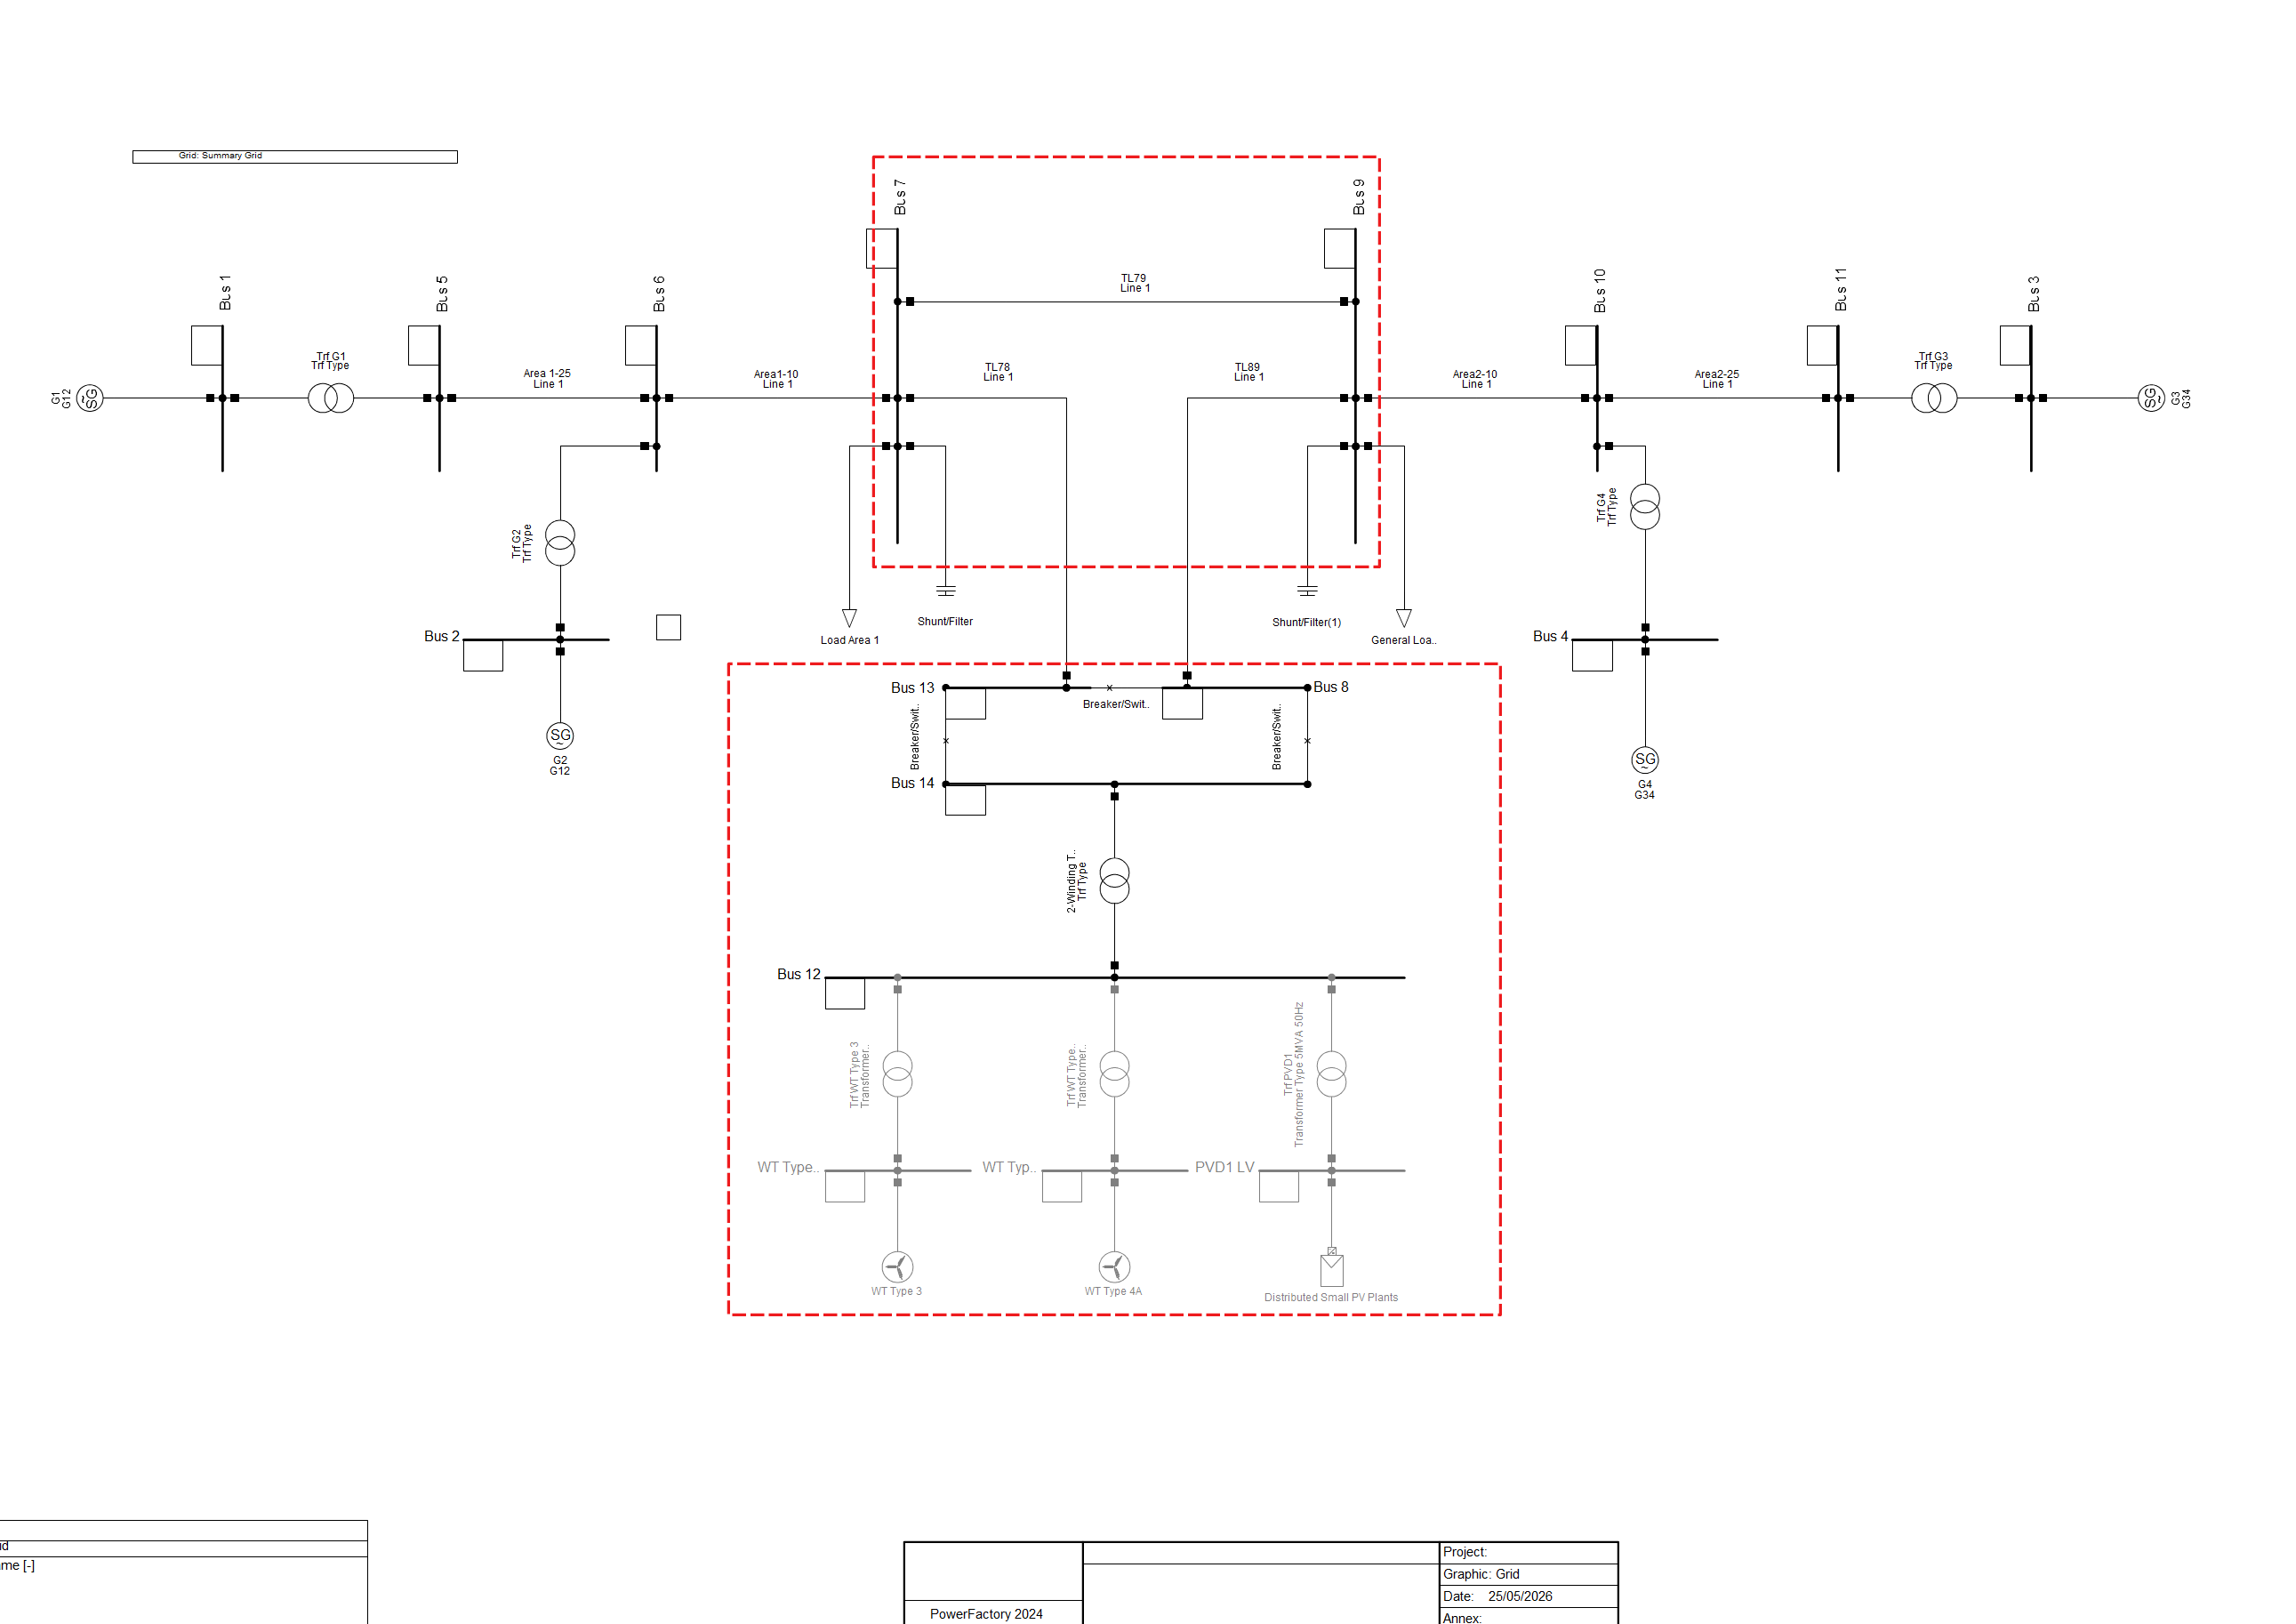
\includegraphics[width=0.8\textwidth]{contents/chapter-3/sld pf.png}
    \caption{\textit{Single line diagram} sistem yang digunakan dalam penelitian}
    \label{fig:sld_pf}
\end{figure}

Model yang digunakan merupakan pengembangan dari sistem awal Kundur two-area. Perubahan utama dilakukan pada nilai \textit{dispatch} beberapa generator dan penyesuaian bagian jaringan di sekitar titik integrasi IBR. Nilai \textit{dispatch} G1 dan G2 yang pada sistem awal sebesar 700 MW masing-masing diubah menjadi 510,5 MW, sedangkan nilai \textit{dispatch} G3 diubah dari 700 MW menjadi 675 MW. Selain itu, konfigurasi Bus 8 dan saluran transmisi di sekitarnya disesuaikan agar integrasi IBR dapat direpresentasikan pada model simulasi. Penyesuaian ini diperlukan agar kondisi dasar, variasi jenis IBR, dan respons proteksi pada saluran yang diamati dapat dibandingkan secara konsisten.

Saluran TL89 yang berada di antara Bus 8 dan Bus 9 digunakan sebagai objek utama proteksi. Pada saluran tersebut dipasang relay dari sisi Bus 8 dan dari sisi Bus 9. Bagian sistem di sekitar TL89 juga terhubung dengan saluran lain, sehingga skenario gangguan internal, gangguan eksternal, dan perubahan konfigurasi jaringan dapat diamati terhadap respons relay.

\begin{figure}[H]
    \centering
    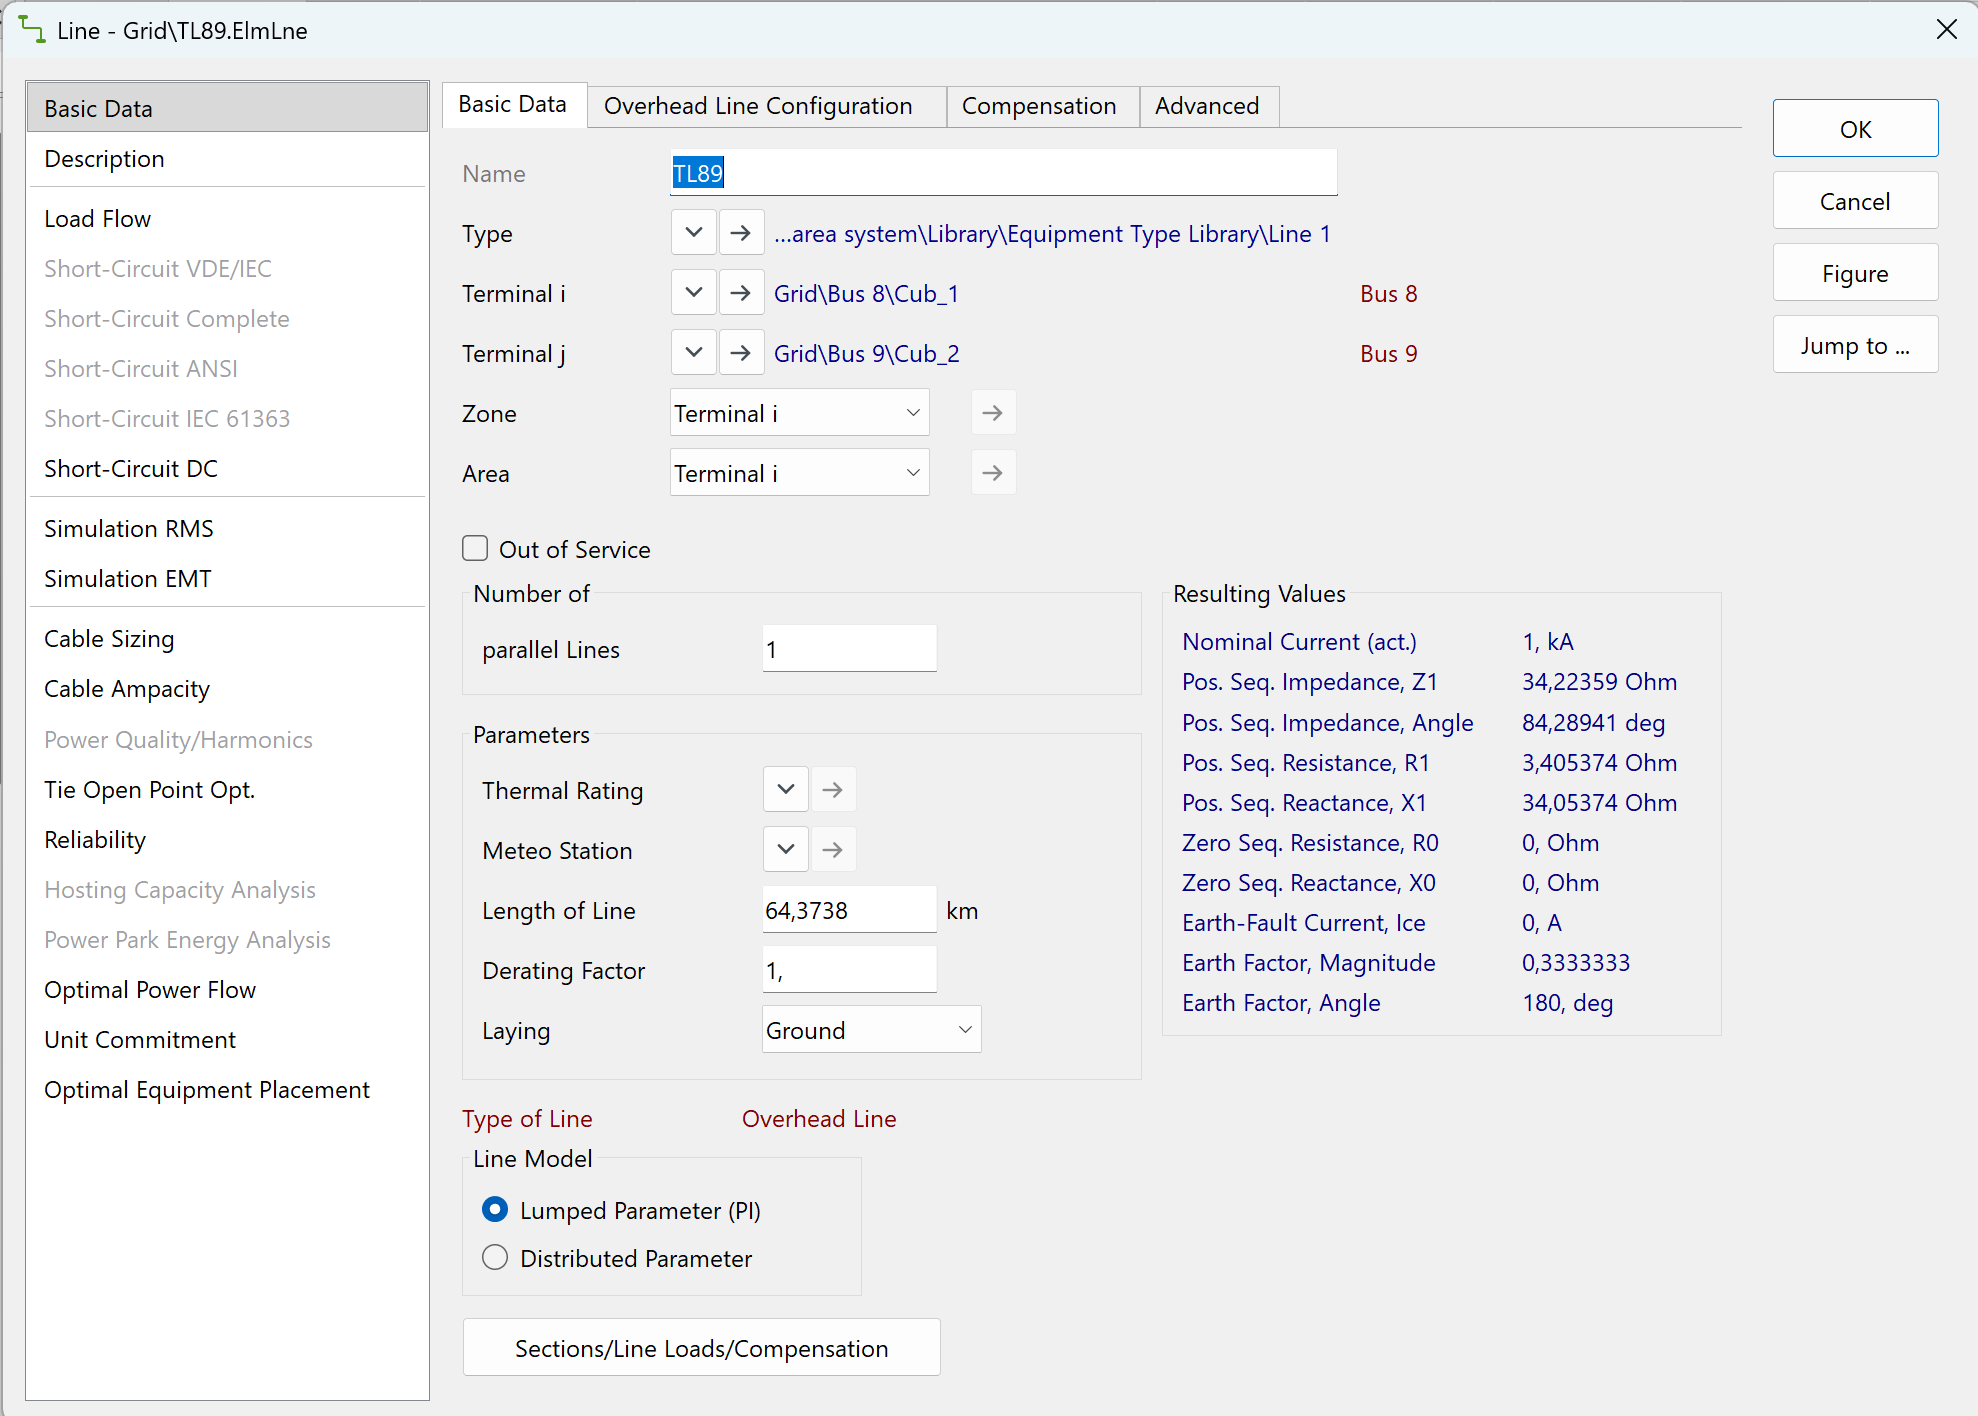
\includegraphics[width=0.95\textwidth]{contents/chapter-3/spesifikasi transmision line.png}
    \caption{Spesifikasi saluran transmisi TL89 pada DIgSILENT PowerFactory}
    \label{fig:spesifikasi_saluran_tl89}
\end{figure}

Spesifikasi saluran TL89 yang digunakan sebagai objek proteksi ditunjukkan pada Gambar \ref{fig:spesifikasi_saluran_tl89}. Berdasarkan data pada gambar tersebut, TL89 menghubungkan terminal Bus 8 dan Bus 9 dengan tipe saluran \textit{overhead line}. Saluran ini memiliki panjang 64,3738 km, jumlah saluran paralel sebanyak satu, serta dimodelkan menggunakan \textit{lumped parameter} \((\pi)\). Nilai yang ditampilkan pada bagian \textit{resulting values} menunjukkan arus nominal sebesar 1 kA, impedansi urutan positif \(Z_1\) sebesar 34,22359 Ohm dengan sudut 84,28941 derajat, resistansi urutan positif \(R_1\) sebesar 3,405374 Ohm, dan reaktansi urutan positif \(X_1\) sebesar 34,05374 Ohm. Parameter ini menjadi dasar pemodelan saluran yang diproteksi sebelum respons relay 21 dan relay 87L diamati pada berbagai skenario gangguan.

Kondisi dasar sistem adalah kondisi sebelum variasi jenis IBR dievaluasi. Kondisi ini digunakan sebagai acuan untuk menyusun setting proteksi konvensional dan sebagai pembanding terhadap hasil simulasi setelah IBR diintegrasikan. Dalam penelitian ini, level penetrasi IBR dibuat tetap sehingga perubahan respons relay tidak ditafsirkan sebagai akibat perubahan kapasitas penetrasi, tetapi sebagai akibat perbedaan karakteristik jenis IBR yang digunakan.

Batas kajian pada model sistem mengikuti batasan penelitian, yaitu evaluasi hanya dilakukan terhadap relay 21 dan relay 87L pada saluran TL89. Analisis tidak mencakup koordinasi proteksi antarrele, skema \textit{main-backup}, maupun optimasi setting proteksi baru.

\section{Pemodelan Sumber Konvensional dan IBR}

Sumber konvensional pada model digunakan untuk merepresentasikan kondisi sistem transmisi sebelum integrasi IBR. Pada kondisi ini, setting relay disusun berdasarkan karakteristik sistem yang masih diasumsikan konvensional. Kondisi tanpa IBR menjadi dasar pembanding untuk melihat perubahan respons relay ketika jenis IBR dimasukkan ke sistem.

IBR yang dibandingkan dalam penelitian ini terdiri atas \textit{wind turbine type 3}, \textit{wind turbine type 4}, dan \textit{photovoltaic}. Ketiga jenis IBR tersebut diperlakukan sebagai variabel utama penelitian. Oleh karena itu, level penetrasi IBR dijaga tetap pada skenario yang dibandingkan, sedangkan jenis sumber IBR yang digunakan diubah sesuai kebutuhan pengujian.

Penamaan skenario IBR pada diagram alir digunakan untuk membedakan kombinasi kondisi pengujian yang dijalankan pada model. Kombinasi tersebut mencakup jenis IBR, lokasi gangguan, jenis gangguan, dan kondisi konfigurasi jaringan yang diuji. Dengan pendekatan ini, hasil simulasi dapat dibandingkan untuk melihat apakah perbedaan jenis IBR menimbulkan perubahan karakteristik operasi relay.

\section{Pemodelan Relay 21 dan Relay 87L}

Relay 21 dimodelkan sebagai proteksi jarak pada saluran TL89. Relay dipasang pada kedua sisi saluran, yaitu sisi Bus 8 dan sisi Bus 9. Respons relay 21 diamati melalui status \textit{pickup}, status \textit{trip}, zona operasi, serta perubahan impedansi tampak yang dibaca relay pada saat gangguan.

Pada penelitian ini, cakupan proteksi relay 21 dibatasi pada dua zona operasi. Zona 1 disusun untuk mencakup 80\% panjang saluran TL89 sebagai proteksi utama dengan cakupan cepat pada saluran yang dilindungi. Zona 2 disusun dengan cakupan 120\% panjang saluran TL89 sehingga dapat menjangkau keseluruhan saluran utama dan sebagian daerah setelah ujung saluran. Pembatasan pada dua zona ini digunakan agar analisis respons relay tetap terfokus pada perubahan impedansi tampak dan keputusan operasi relay terhadap skenario gangguan yang diuji.

Relay 87L dimodelkan sebagai proteksi \textit{differential} saluran pada TL89. Sama seperti relay 21, relay 87L ditempatkan pada kedua sisi saluran, yaitu sisi Bus 8 dan sisi Bus 9. Respons relay 87L diamati melalui status operasi relay serta hubungan antara arus \textit{differential} dan arus \textit{restraint}.

Besaran arus dan tegangan yang digunakan oleh relay diperoleh melalui transformator instrumen yang terpasang pada model. Rasio CT yang digunakan adalah 5:1000, sedangkan rasio VT yang digunakan adalah 115:230000. Jenis VT yang digunakan pada pemodelan ini adalah \textit{ideal voltage transformer}. Penggunaan rasio CT dan VT tersebut menjadi dasar pembacaan besaran sekunder oleh relay sebelum nilai impedansi tampak, arus diferensial, dan arus \textit{restraint} dianalisis pada skenario gangguan.

Setting relay 21 disesuaikan berdasarkan kondisi sistem konvensional, yaitu kondisi sebelum integrasi IBR. Dengan demikian, evaluasi relay 21 diarahkan untuk melihat apakah setting tersebut masih memberikan respons yang sesuai ketika jenis IBR diubah. Untuk relay 87L, pengujian menggunakan setting bawaan atau \textit{default} yang tersedia pada model. Kedua relay dianalisis secara individual sehingga hasil penelitian tidak ditafsirkan sebagai kajian koordinasi proteksi.

\section{Penentuan Skenario Pengujian}

Skenario pengujian disusun untuk membandingkan respons relay pada kondisi tanpa IBR dan kondisi dengan integrasi IBR. Kondisi tanpa IBR digunakan sebagai acuan awal, sedangkan kondisi dengan IBR dikelompokkan berdasarkan jenis IBR yang digunakan, yaitu \textit{wind turbine type 3}, \textit{wind turbine type 4}, dan \textit{photovoltaic}.

Selain berdasarkan jenis IBR, skenario juga mempertimbangkan lokasi gangguan. Gangguan diuji pada saluran yang menjadi objek proteksi dan pada saluran lain di luar objek proteksi. Pemisahan ini diperlukan agar respons relay dapat dibedakan antara gangguan internal dan gangguan eksternal terhadap zona proteksi yang diamati.

Skenario juga mencakup kondisi salah satu saluran transmisi \textit{out of service}. Kondisi ini digunakan untuk melihat perubahan respons relay ketika konfigurasi jaringan berubah. Jenis gangguan yang digunakan pada hasil awalmencakup gangguan satu fasa ke tanah, gangguan dua fasa ke tanah, dan gangguan tiga fasa. Pengelompokan skenario tersebut digunakan agar hasil simulasi dapat dianalisis secara konsisten pada setiap jenis IBR.

Rincian skenario pengujian yang digunakan pada penelitian ini ditunjukkan pada Tabel \ref{tab:skenario_gangguan_ibr}. Tabel tersebut merangkum kombinasi jenis IBR, jenis gangguan, lokasi gangguan, dan kondisi kontingensi saluran yang digunakan pada simulasi. Penyajian skenario dalam bentuk tabel diperlukan agar setiap hasil simulasi pada bab pembahasan dapat ditelusuri kembali ke kondisi pengujian yang sama.

\begin{table}[H]
    \centering
    \caption{Skenario Gangguan pada Sistem dengan Integrasi IBR}
    \label{tab:skenario_gangguan_ibr}
    \resizebox{\textwidth}{!}{%
        \begin{tabular}{|c|c|c|l|}
            \hline
            \textbf{Skenario} & \textbf{Jenis IBR}  & \textbf{Jenis Gangguan} & \textbf{Location and Contingency}                             \\ \hline
            1                 & Wind Turbine Type 3 & DLG                     & Gangguan pada TL89 dekat dengan bus 2 dan TL79 out of service \\ \hline
            2                 & Wind Turbine Type 4 & DLG                     & Gangguan pada TL79 dekat dengan bus 9 dan TL78 out of service \\ \hline
            3                 & Wind Turbine Type 3 & DLG                     & Gangguan pada TL79 dekat dengan bus 9 dan TL78 out of service \\ \hline
            4                 & Wind Turbine Type 3 & 3P                      & Gangguan pada TL79 dekat dengan bus 9 dan TL78 out of service \\ \hline
            5                 & Wind Turbine Type 3 & SLG                     & Gangguan pada TL79 dekat dengan bus 9 dan TL78 out of service \\ \hline
            6                 & Photovoltaic        & DLG                     & Gangguan pada TL79 dekat dengan bus 9 dan TL78 out of service \\ \hline
        \end{tabular}%
    }
\end{table}

Berdasarkan Tabel \ref{tab:skenario_gangguan_ibr}, skenario pertama digunakan untuk mengamati gangguan pada saluran TL89 sebagai objek proteksi utama. Skenario berikutnya digunakan untuk mengamati pengaruh gangguan pada TL79 dengan kondisi TL78 \textit{out of service}. Susunan ini membuat respons relay pada TL89 dapat dibandingkan antara kondisi gangguan pada saluran yang diproteksi dan gangguan pada saluran lain di sekitar objek proteksi. Perbedaan jenis IBR pada skenario tersebut kemudian menjadi dasar untuk menilai apakah karakteristik operasi relay berubah ketika sumber IBR yang terhubung ke sistem diganti.

\section{Parameter dan Indikator Evaluasi}

Parameter utama untuk relay 21 adalah status \textit{pickup}, status \textit{trip}, zona operasi, dan impedansi tampak. Impedansi tampak digunakan untuk melihat posisi titik operasi relay terhadap karakteristik zona proteksi. Pergeseran titik impedansi tampak menjadi indikator adanya perubahan karakteristik operasi relay akibat perubahan sumber gangguan pada sistem.

Parameter utama untuk relay 87L adalah status \textit{pickup}, status \textit{trip}, arus diferensial, dan arus \textit{restraint}. Hubungan antara arus diferensial dan arus \textit{restraint} digunakan untuk menilai apakah relay berada pada daerah operasi atau daerah penahan. Jika data waktu operasi tersedia dari hasil simulasi, waktu operasi digunakan sebagai parameter pendukung.

Indikator evaluasi pada penelitian ini adalah kesesuaian respons relay terhadap jenis gangguan dan lokasi gangguan. Untuk relay 21, indikator tersebut dilihat dari apakah impedansi tampak berada pada zona yang sesuai dan apakah relay mengalami kondisi seperti \textit{overreach}, \textit{underreach}, \textit{dropout}, atau trip yang tidak semestinya. Untuk relay 87L, indikatornya dilihat dari kecenderungan arus diferensial dan arus \textit{restraint} terhadap keputusan operasi relay.

\section{Prosedur Simulasi dan Pengambilan Data}

Prosedur simulasi diawali dengan menjalankan model pada kondisi dasar tanpa IBR. Kondisi ini digunakan untuk memastikan bahwa model sistem dan relay dapat digunakan sebagai acuan awal. Setelah itu, setting relay 21 disusun berdasarkan kondisi konvensional, sedangkan relay 87L menggunakan setting \textit{default} pada model.

Tahap berikutnya adalah menjalankan skenario dengan integrasi IBR. Jenis IBR diganti sesuai kelompok pengujian yang telah ditentukan, yaitu \textit{wind turbine type 3}, \textit{wind turbine type 4}, dan \textit{photovoltaic}. Pada setiap kelompok, gangguan diterapkan sesuai skenario lokasi dan jenis gangguan. Jika skenario membutuhkan perubahan konfigurasi jaringan, salah satu saluran transmisi dibuat \textit{out of service} sebelum simulasi gangguan dijalankan.

Data yang diambil dari simulasi meliputi respons operasi relay dan besaran listrik yang menjadi dasar evaluasi. Untuk relay 21, data yang dikumpulkan mencakup impedansi tampak dan keputusan operasi relay. Untuk relay 87L, data yang dikumpulkan mencakup arus diferensial, arus \textit{restraint}, dan keputusan operasi relay. Hasil setiap skenario kemudian disimpan untuk dianalisis dan dibandingkan antarjenis IBR.

\section{Metode Analisis Hasil}

Analisis hasil dilakukan secara kualitatif dan komparatif. Analisis kualitatif digunakan untuk menjelaskan perubahan perilaku relay pada setiap skenario, sedangkan analisis komparatif digunakan untuk membandingkan respons relay pada \textit{wind turbine type 3}, \textit{wind turbine type 4}, dan \textit{photovoltaic}.

Untuk relay 21, analisis difokuskan pada perubahan impedansi tampak dan keputusan operasi relay. Titik impedansi tampak dibandingkan terhadap karakteristik zona proteksi untuk mengidentifikasi apakah relay bekerja sesuai ekspektasi, mengalami \textit{overreach}, mengalami \textit{underreach}, mengalami \textit{dropout}, atau menunjukkan trip yang tidak semestinya.

Untuk relay 87L, analisis difokuskan pada hubungan antara arus diferensial dan arus \textit{restraint}. Perubahan hubungan kedua besaran tersebut digunakan untuk melihat apakah integrasi IBR memengaruhi kecenderungan operasi relay diferensial saluran. Hasil analisis relay 21 dan relay 87L kemudian disintesiskan untuk mengevaluasi kelayakan penggunaan setting konvensional pada sistem transmisi dengan IBR.

Agar tahapan analisis relay 21 dapat dijelaskan secara lebih rinci, alur perhitungan impedansi tampak ditunjukkan pada Gambar \ref{fig:flowchart_impedansi_tampak_relay21}. Diagram alir tersebut memperlihatkan bahwa analisis relay 21 tidak hanya melihat keputusan \textit{pickup} dan \textit{trip}, tetapi juga menelusuri besaran tegangan dan arus yang digunakan untuk membentuk nilai impedansi tampak pada masing-masing elemen gangguan.

\usetikzlibrary{shapes.geometric, arrows.meta, positioning}

\begin{figure}[H]
    \centering
    \resizebox{0.42\textwidth}{!}{%
        \begin{tikzpicture}[
            node distance=1.1cm,
            every node/.style={font=\small},
            startstop/.style={
                    ellipse,
                    draw,
                    minimum width=3.0cm,
                    minimum height=1.0cm,
                    align=center
                },
            process/.style={
                    rectangle,
                    draw,
                    minimum width=4.4cm,
                    minimum height=1.15cm,
                    align=center
                },
            data/.style={
                    trapezium,
                    trapezium left angle=70,
                    trapezium right angle=110,
                    draw,
                    minimum width=5.0cm,
                    minimum height=1.2cm,
                    align=center
                },
            arrow/.style={
            -{Latex[length=2.5mm]},
            thick
            }
            ]

            % Node flowchart
            \node (start) [startstop] {START};

            \node (data) [data, below=of start] {
                Pengambilan Data\\[1mm]
                $V_A, V_B, V_C, I_A, I_B, I_C, 3I_0,$ dan $k_0$
            };

            \node (zab) [process, below=of data] {
                Hitung Nilai $Z_{AB}$ :\\[1mm]
                $Z_{AB}=\dfrac{V_A-V_B}{I_A-I_B}$
            };

            \node (zbc) [process, below=of zab] {
                Hitung Nilai $Z_{BC}$ :\\[1mm]
                $Z_{BC}=\dfrac{V_B-V_C}{I_B-I_C}$
            };

            \node (zca) [process, below=of zbc] {
                Hitung Nilai $Z_{CA}$ :\\[1mm]
                $Z_{CA}=\dfrac{V_C-V_A}{I_C-I_A}$
            };

            \node (zag) [process, below=of zca] {
                Hitung Nilai $Z_{AG}$ :\\[1mm]
                $Z_{AG}=\dfrac{V_A}{I_A+k_0(3I_0)}$
            };

            \node (zbg) [process, below=of zag] {
                Hitung Nilai $Z_{BG}$ :\\[1mm]
                $Z_{BG}=\dfrac{V_B}{I_B+k_0(3I_0)}$
            };

            \node (ambil) [process, below=of zbg, minimum height=1.35cm] {Ambil hasil perhitungan sesuai\\dengan jenis gangguan};

            \node (analisis) [process, below=of ambil, minimum height=1.35cm] {Analisis impedansi tampak\\untuk relay 21};

            \node (end) [startstop, below=of analisis] {END};

            % Garis panah
            \draw [arrow] (start) -- (data);
            \draw [arrow] (data) -- (zab);
            \draw [arrow] (zab) -- (zbc);
            \draw [arrow] (zbc) -- (zca);
            \draw [arrow] (zca) -- (zag);
            \draw [arrow] (zag) -- (zbg);
            \draw [arrow] (zbg) -- (ambil);
            \draw [arrow] (ambil) -- (analisis);
            \draw [arrow] (analisis) -- (end);

        \end{tikzpicture}%
    }
    \caption{Flowchart Perhitungan Impedansi Tampak untuk Relay 21}
    \label{fig:flowchart_impedansi_tampak_relay21}
\end{figure}

Berdasarkan Gambar \ref{fig:flowchart_impedansi_tampak_relay21}, proses analisis dimulai dari pengambilan data tegangan fasa, arus fasa, arus urutan nol, dan faktor kompensasi urutan nol. Data tersebut kemudian digunakan untuk menghitung impedansi tampak pada elemen gangguan satu fasa ke tanah dan elemen gangguan antarfasa. Nilai impedansi yang digunakan dalam analisis dipilih sesuai dengan jenis gangguan pada skenario pengujian, misalnya elemen fasa-tanah untuk gangguan satu fasa ke tanah dan elemen antarfasa untuk gangguan antar fasa.

Hasil perhitungan impedansi tampak kemudian dibandingkan dengan karakteristik zona proteksi relay 21. Perbandingan ini digunakan untuk menilai apakah titik operasi relay berada pada zona yang sesuai atau menunjukkan penyimpangan seperti \textit{overreach}, \textit{underreach}, \textit{dropout}, atau trip yang tidak semestinya. Dengan demikian, diagram alir tersebut menjadi rincian teknis dari metode analisis kualitatif dan komparatif yang digunakan untuk mengevaluasi respons relay 21 pada setiap skenario IBR.
